\chapter{Model liniowy}
\section{Równania stanu}
W celu opracowania modelu liniowego obiektu wykonaliśmy linearyzację w zadanym punkcie pracy. Pamiętając, że pochodna w tym punkcie wynosi 0, otrzymaliśmy następujące równania:

\begin{equation}
\left\{
\begin{tabular}{l}
$\frac{dC_A}{dt} = (-1-10^{10}\cdot e^{-\frac{8330.1}{T_0}})(C_A-C_{A0})+(-10^{10}\cdot e^{-\frac{8330.1}{T_0}}\cdot \frac{8330.1}{T_0^2}\cdot C_{A0})(T-T_0)+(C_{Ain}-C_{Ain0})$\\\\
$\frac{dT}{dt} = (130\cdot 10^{10}\cdot e^{-\frac{8330.1}{T_0}})(C_A-C_{A0}) + (-1+130\cdot 10^{10}\cdot e^{-\frac{8330.1}{T_0}}\cdot \frac{8330.1}{T_0^2}\cdot C_{A0}-\frac{1.678\cdot (F_C)^{1.5}}{F_C+0.839\cdot (F_C)^{0.5}})(T-T_0)$\\\\
$\quad + (-1.678(T_0-T_{Cin0})(\frac{1.5\cdot (F_{C0})^{0.5}}{F_{C0}+0.839\cdot (F_{C0})^{0.5}}-\frac{ (F_{C0})^{1.5}}{(F_{C0}+0.839\cdot (F_{C0})^{0.5})^2}\cdot (1+0.5\cdot 0.839 \cdot (F_{C0})^{-0.5})))(F_C-F_{C0})$\\\\
$\quad + (T_{in} - T_{in0}) + (\frac{1.678\cdot (F_C)^{1.5}}{F_C+0.839\cdot (F_C)^{0.5}})(T_{Cin} - T_{Cin0})$\\\\
\end{tabular}
\right.
\end{equation}
Podstawiając wartości w punkcie pracy (zmienne z indeksem 0) otrzymujemy:
\begin{equation}
\left\{
\begin{tabular}{l}
$\frac{dC_A}{dt} = -7.5597(C_A-0.2646)-0.0932(T-393.9531)+(C_{Ain}-2)$\\\\
$\frac{dT}{dt} = 852.7638(C_A-0.2646) + 5.7693(T-393.9531) -6.0732(F_C-15) + (T_{in} - 323) + 5.3417(T_{Cin} - 365)$\\\\
\end{tabular}
\right.
\end{equation}

\begin{equation}
\left\{
\begin{tabular}{l}
$\frac{dC_A}{dt} = -7.5597\cdot C_A-0.0932\cdot T+C_{Ain} + 36.7167$\\\\
$\frac{dT}{dt} = 852.7638\cdot C_A + 5.7693\cdot T -6.0732\cdot F_C + T_{in} + 5.3417\cdot T_{Cin} - 4680.0974$\\\\
\end{tabular}
\right.
\end{equation}
\newpage
\section{Transmitancja}
Mając model w postaci układu równań wykorzystaliśmy możliwości Matlaba do stworzenia obiektu reprezentującego te równania (obiekt $ss()$), a następnie obliczania transmitancji (obiekt $tf()$). Macierze równań stanu mają następującą postać:
\begin{equation}
	A=\left[
	\begin{tabular}{c c}
	-7.5597&-0.0932\\852.7638&5.7693
	\end{tabular}
	\right]
\end{equation}
\begin{equation}
B=\left[
\begin{tabular}{c c c c}
1&0&0&0\\0&-6.0732&1&5.3417
\end{tabular}
\right]
\end{equation}
\begin{equation}
C=\left[
\begin{tabular}{c c}
1&0\\0&1
\end{tabular}
\right]
\end{equation}
\begin{equation}
D=\left[
\begin{tabular}{c c c c}
0&0&0&0\\0&0&0&0
\end{tabular}
\right]
\end{equation}
Wyliczone transmitancje to:
\begin{equation}
	\frac{C_A(s)}{C_{Ain}(s)} = \frac{s-5.769}{s^2+1.79s+35.83}
\end{equation}
\begin{equation}
\frac{C_A(s)}{F_C(s)} = \frac{0.5658}{s^2+1.79s+35.83}
\end{equation}
\begin{equation}
\frac{C_A(s)}{T_{in}(s)} = \frac{-0.09316}{s^2+1.79s+35.83}
\end{equation}
\begin{equation}
\frac{C_A(s)}{T_{Cin}(s)} = \frac{-0.4976}{s^2+1.79s+35.83}
\end{equation}
\begin{equation}
\frac{T(s)}{C_{Ain}(s)} = \frac{8.52.8}{s^2+1.79s+35.83}
\end{equation}
\begin{equation}
\frac{T(s)}{F_C(s)} = \frac{-6.073s-45.91}{s^2+1.79s+35.83}
\end{equation}
\begin{equation}
\frac{T(s)}{T_{in}(s)} = \frac{s + 7.56}{s^2+1.79s+35.83}
\end{equation}
\begin{equation}
\frac{T(s)}{T_{Cin}(s)} = \frac{5.342 s + 40.38}{s^2+1.79s+35.83}
\end{equation}
\newpage
\section{Porównanie modelu nieliniowego i liniowego}
Po zaimplementowaniu modelu w postaci równań stanu w Matlabie, wykonaliśmy eksperymenty polegające na zmianie wartości jednej ze zmiennych sterujących. Na wykresach od \ref{fig:lincacain0} do \ref{fig:lintfc0} przedstawione zostały przebiegi wyjść dla małych zmian zmiennych sterujących. Jak widać model ten radzi sobie w tym zakresie zadowalająco. Odchyły stężenia $C_A$ względem modelu nieliniowego nie są duże, i mieszczą się w zakresie $<-0.01;0.01>$. Różnica temperatury $T$ między modelami nie przekracza jednego stopnia Kelwina. Przebiegi dla obydwu modeli są także podobne kształtem.

Inaczej przedstawia się sytuacja dla dużych skoków sterowania, przedstawiona na wykresach od \ref{fig:lincacain1} do \ref{fig:lintfc1}. Odchylenie modelu liniowego od nieliniowego jest ewidentnie większe, i w większości przypadków kształt przebiegów nie pokrywa się pomiędzy modelami. Szczególną uwagę należy zwrócić jednak na wykres \ref{fig:lintcain1}, ponieważ tylko na nim wartość końcowa wyjścia $T$ modelu liniowego jest zbliżona do wartości dla modelu nieliniowego. Oznacza to, że w teorii model liniowy powinien dosyć dobrze odwzorowywać wartość wyjścia $T$ przy skokach sterowania $C_{Ain}$.

\begin{figure}
	\centering
	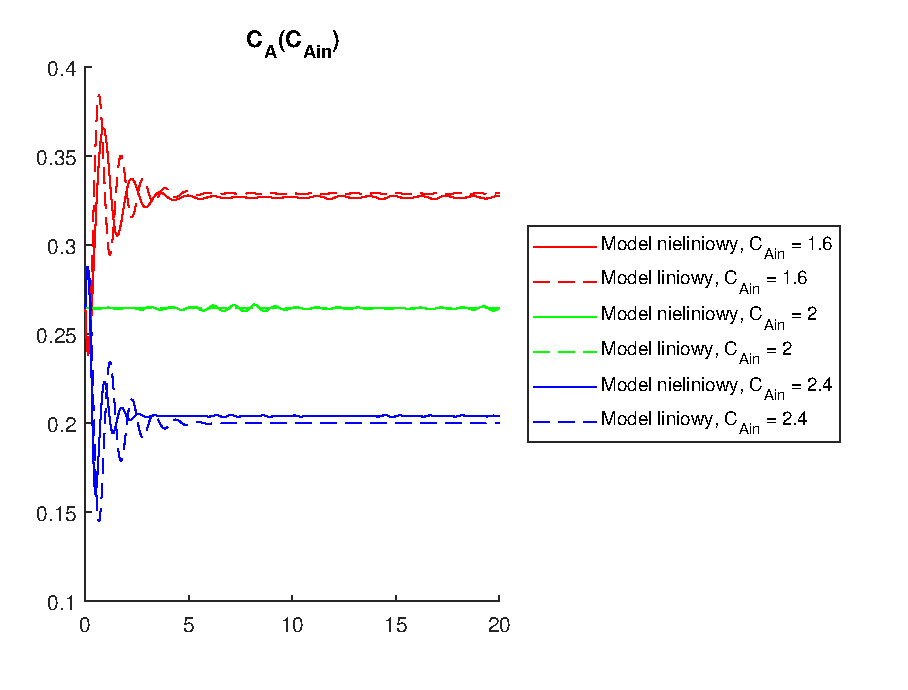
\includegraphics[width=.8\linewidth]{plot/lin_cacain_0.eps}
	\caption{Porównanie wyjścia $C_A$ modelu nieliniowego i liniowego dla skoku sterowania $C_{Ain}$ blisko punktu pracy}
	\label{fig:lincacain0}
\end{figure}
\begin{figure}
\centering
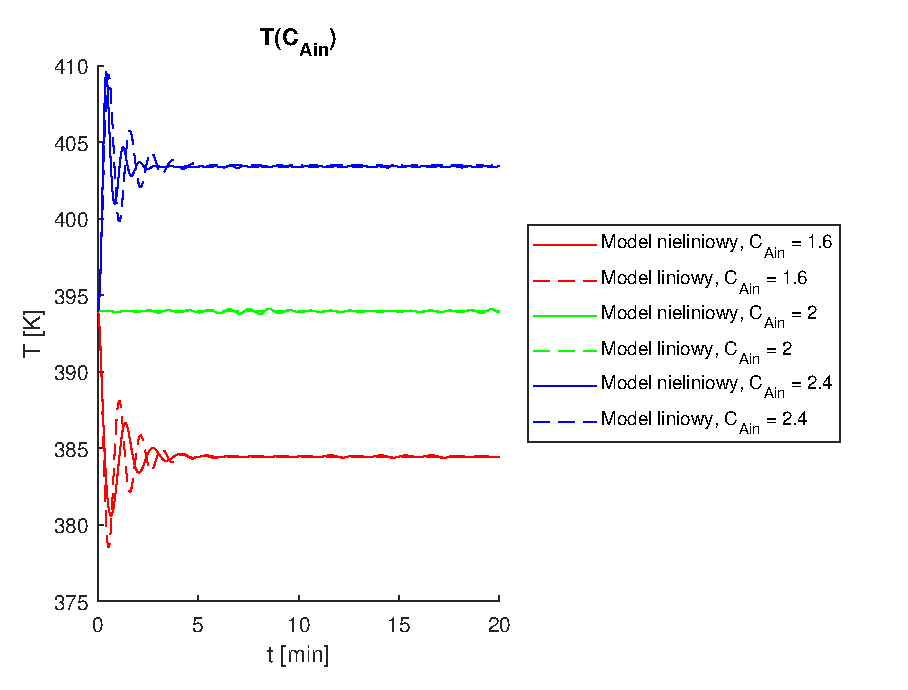
\includegraphics[width=.8\linewidth]{plot/lin_tcain_0.eps}
\caption{Porównanie wyjścia $T$ modelu nieliniowego i liniowego dla skoku sterowania $C_{Ain}$ blisko punktu pracy}
\label{fig:lintcain0}
\end{figure}
\begin{figure}
\centering
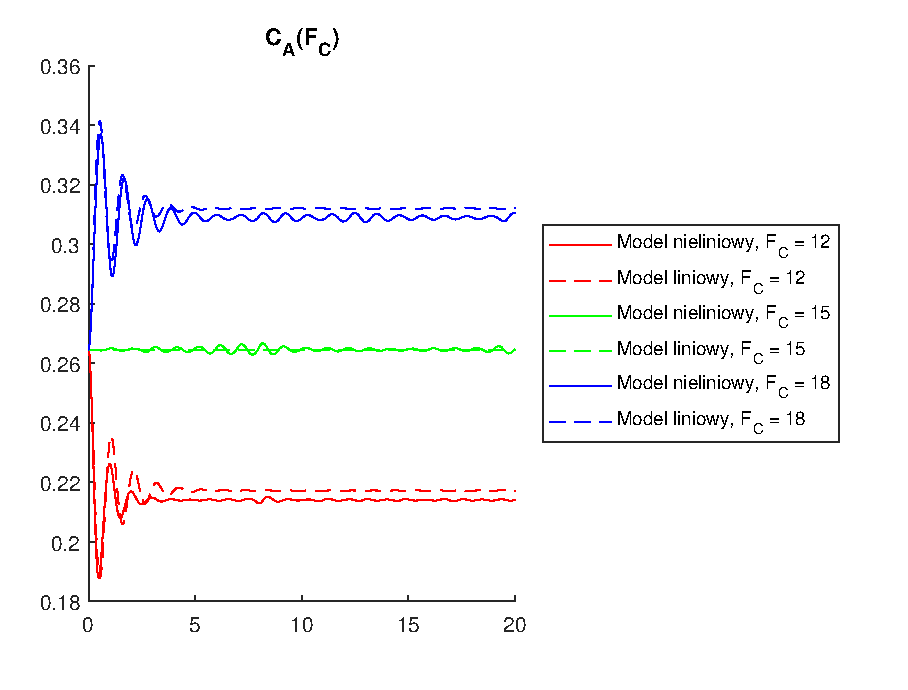
\includegraphics[width=.8\linewidth]{plot/lin_cafc_0.eps}
\caption{Porównanie wyjścia $C_A$ modelu nieliniowego i liniowego dla skoku sterowania $F_C$ blisko punktu pracy}
\label{fig:lincafc0}
\end{figure}
\begin{figure}
\centering
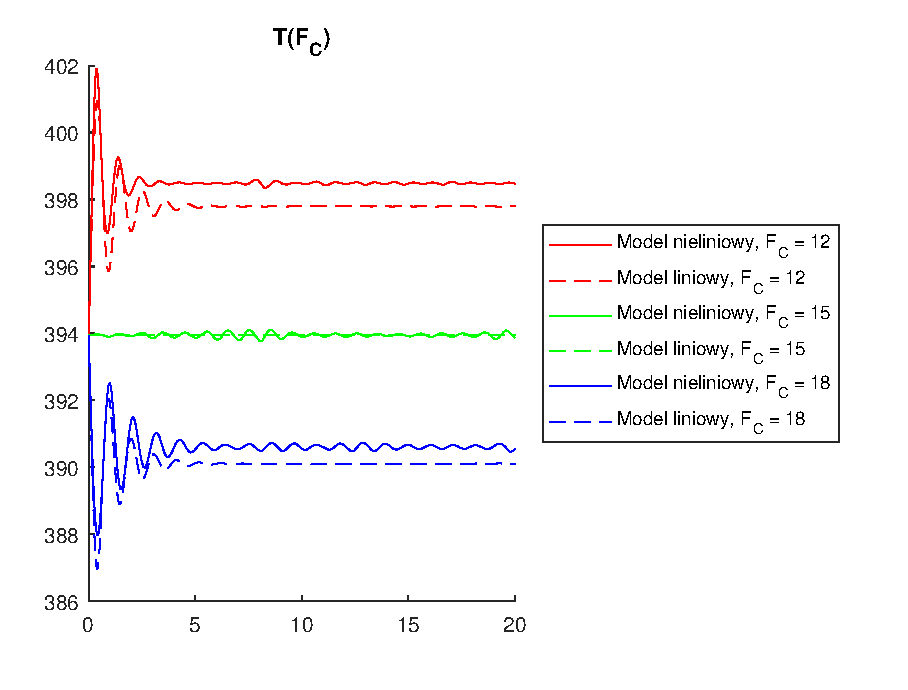
\includegraphics[width=.8\linewidth]{plot/lin_tfc_0.eps}
\caption{Porównanie wyjścia $T$ modelu nieliniowego i liniowego dla skoku sterowania $F_C$ blisko punktu pracy}
\label{fig:lintfc0}
\end{figure}

\begin{figure}
	\centering
	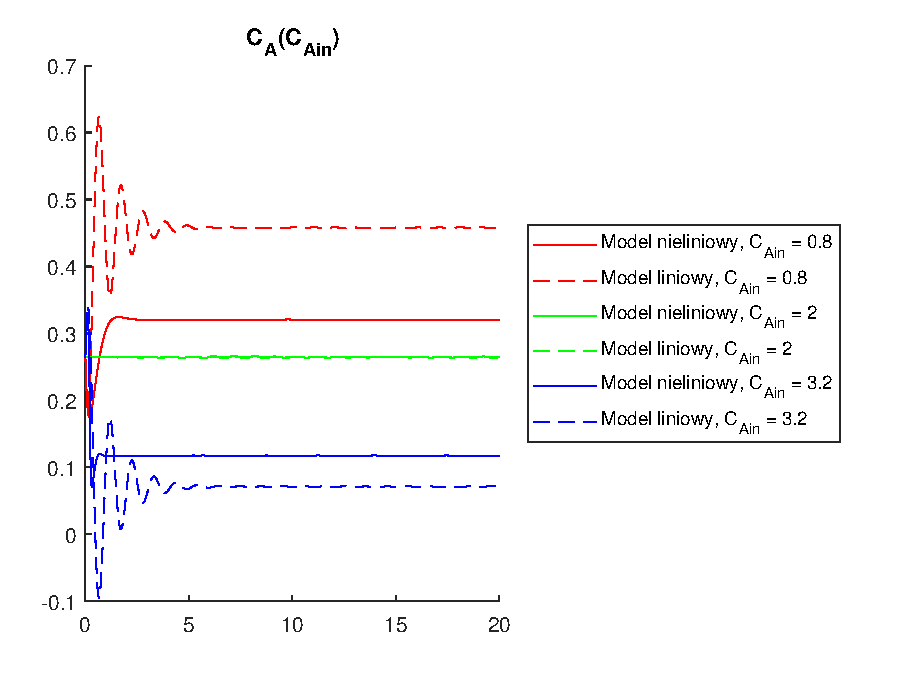
\includegraphics[width=.8\linewidth]{plot/lin_cacain_1.eps}
	\caption{Porównanie wyjścia $C_A$ modelu nieliniowego i liniowego dla skoku sterowania $C_{Ain}$ daleko od punktu pracy}
	\label{fig:lincacain1}
\end{figure}
\begin{figure}
	\centering
	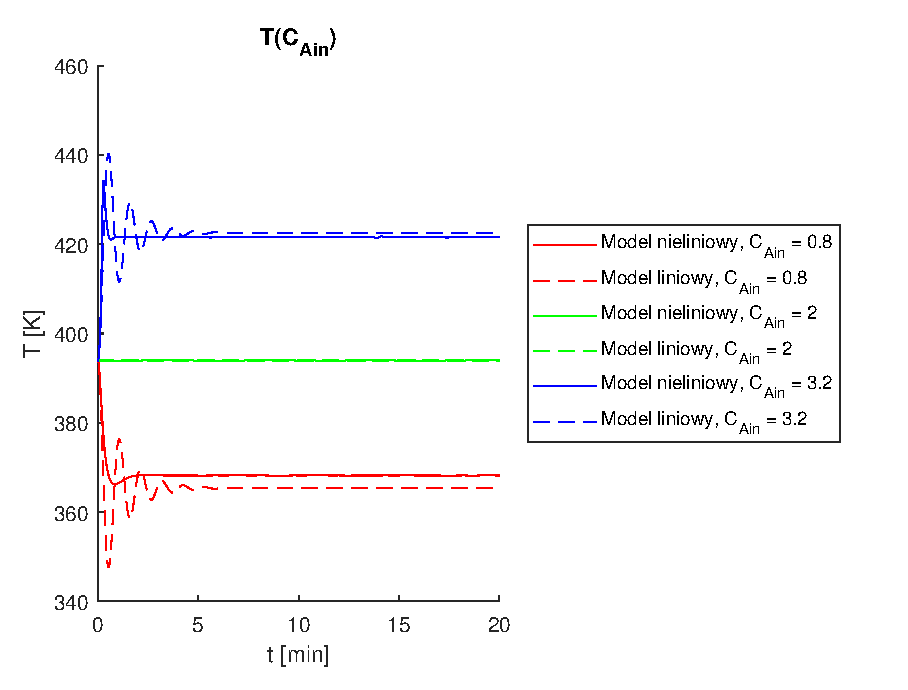
\includegraphics[width=.8\linewidth]{plot/lin_tcain_1.eps}
	\caption{Porównanie wyjścia $T$ modelu nieliniowego i liniowego dla skoku sterowania $C_{Ain}$ daleko od punktu pracy}
	\label{fig:lintcain1}
\end{figure}
\begin{figure}
	\centering
	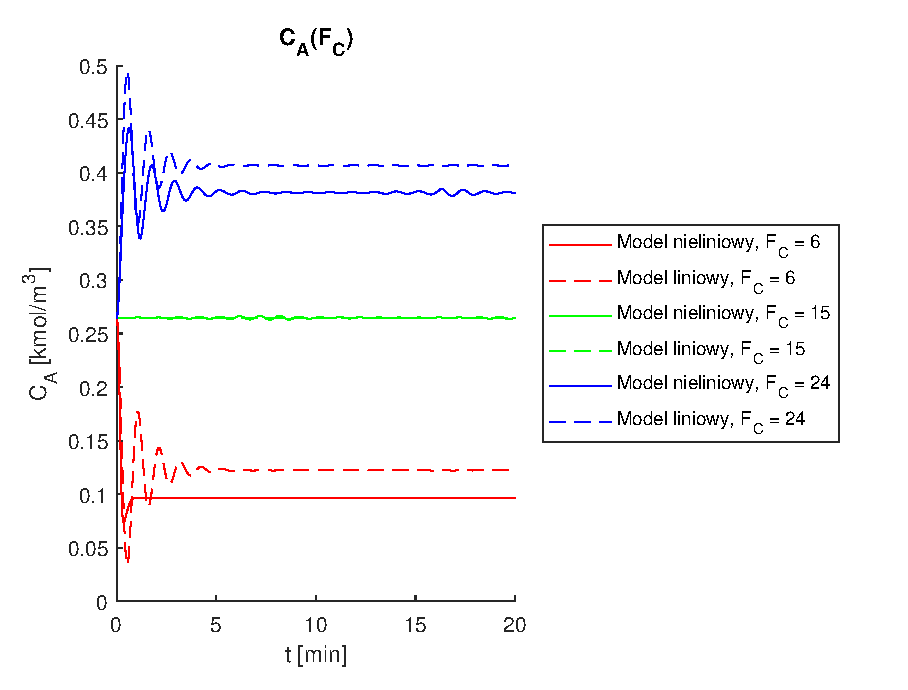
\includegraphics[width=.8\linewidth]{plot/lin_cafc_1.eps}
	\caption{Porównanie wyjścia $C_A$ modelu nieliniowego i liniowego dla skoku sterowania $F_C$ daleko od punktu pracy}
	\label{fig:lincafc1}
\end{figure}
\begin{figure}
	\centering
	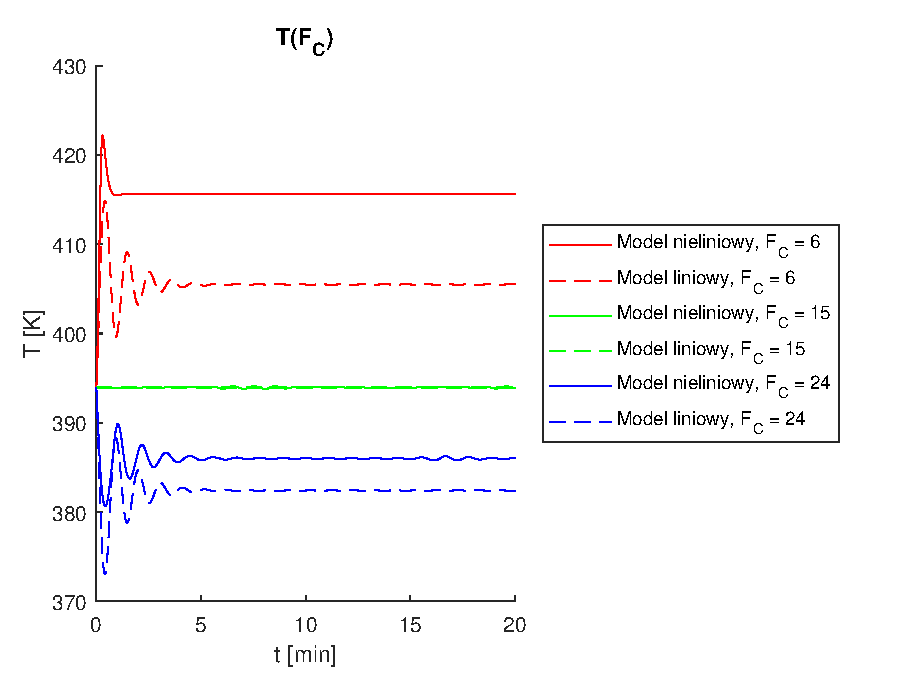
\includegraphics[width=.8\linewidth]{plot/lin_tfc_1.eps}
	\caption{Porównanie wyjścia $T$ modelu nieliniowego i liniowego dla skoku sterowania $F_C$ daleko od punktu pracy}
	\label{fig:lintfc1}
\end{figure}
